\documentclass{report}
\usepackage{amsmath}
\usepackage{tikz}
\usepackage[section]{placeins}
\usetikzlibrary{automata, arrows.meta, positioning}



\setcounter{chapter}{+1}

\title{Language and Automata, Assignment 1}
\author{Krzysztof Rudnicki\\ Student number: 307585}
\date{\today}


\begin{document}
\maketitle

\section{Regular expression}
We are given following regular expression:
\[ a^* + ba^*b + bba^*\]

\section{Examples of accepted strings}
\begin{enumerate}
\item $ \varepsilon $
\item a
\item bab
\item bba
\item bb
\end{enumerate}

\section{Building NFA using Thompson construction algorithm}
\begin{figure}[!htb]
\centering
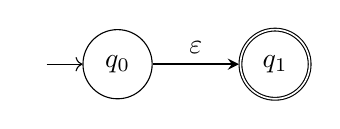
\begin{tikzpicture} [node distance = 2cm, on grid, auto]

\node (q0) [state, initial, initial text = {}] {$q_0$};
\node (q1) [state, accepting, right = of q0] {$q_1$};

\path [-stealth, thick]
    (q0) edge node {$\varepsilon$}   (q1);
\end{tikzpicture}
\caption{Operator 'a'} \label{fig:operatorA}
\end{figure}

\begin{figure}[!htb]
\centering
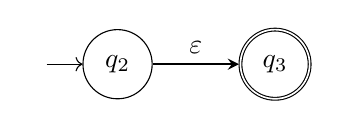
\begin{tikzpicture} [node distance = 2cm, on grid, auto]

\node (q0) [state, initial, initial text = {}] {$q_2$};
\node (q1) [state, accepting, right = of q0] {$q_3$};

\path [-stealth, thick]
    (q0) edge node {$\varepsilon$}   (q1);
\end{tikzpicture}
\caption{Operator 'b'} \label{fig:operatorB}
\end{figure}

\begin{figure}[!htb]
\centering
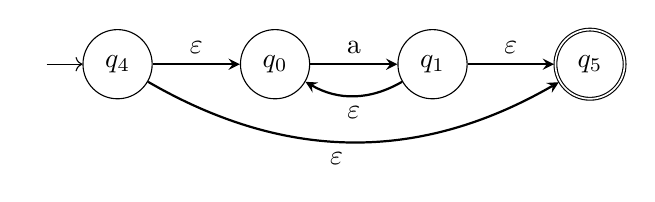
\begin{tikzpicture} [node distance = 2cm, on grid, auto]

\node (q0) [state, initial, initial text = {}] {$q_4$};
\node (q1) [state, right = of q0] {$q_0$};
\node (q2) [state, right = of q1] {$q_1$};
\node (q3) [state, accepting, right = of q2] {$q_5$};

\path [-stealth, thick]
    (q0) edge node {$\varepsilon$}   (q1);
\path [-stealth, thick]
    (q0) edge [bend right] node[below left] {$\varepsilon$}   (q3);
\path [-stealth, thick]
    (q1) edge node {a}   (q2);
\path [-stealth, thick]
    (q2) [bend left] edge node {$\varepsilon$}   (q1);
\path [-stealth, thick]
    (q2) edge node {$\varepsilon$}   (q3);
\end{tikzpicture}
\caption{Operator '$a^*$'} \label{fig:operatorAstar}
\end{figure}

\begin{figure}[!htb]
\centering
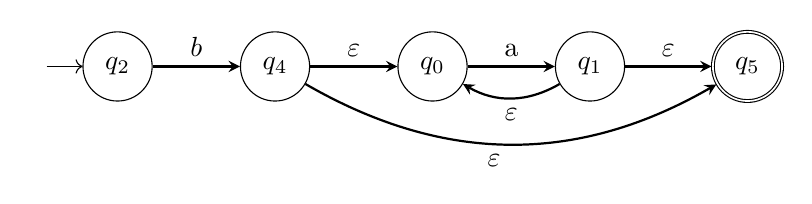
\begin{tikzpicture} [node distance = 2cm, on grid, auto]

\node (q6) [state, initial, initial text = {}] {$q_2$};
\node (q0) [state, right = of q6] {$q_4$};
\node (q1) [state, right = of q0] {$q_0$};
\node (q2) [state, right = of q1] {$q_1$};
\node (q3) [state, accepting, right = of q2] {$q_5$};

\path [-stealth, thick]
        (q6) edge node {$b$}   (q0);
\path [-stealth, thick]
    (q0) edge node {$\varepsilon$}   (q1);
\path [-stealth, thick]
    (q0) edge [bend right] node[below left] {$\varepsilon$}   (q3);
\path [-stealth, thick]
    (q1) edge node {a}   (q2);
\path [-stealth, thick]
    (q2) [bend left] edge node {$\varepsilon$}   (q1);
\path [-stealth, thick]
    (q2) edge node {$\varepsilon$}   (q3);
\end{tikzpicture}
\caption{Operator '$ba^*$'} \label{fig:operatorbastar}
\end{figure}

\begin{figure}[!htb]
\centering
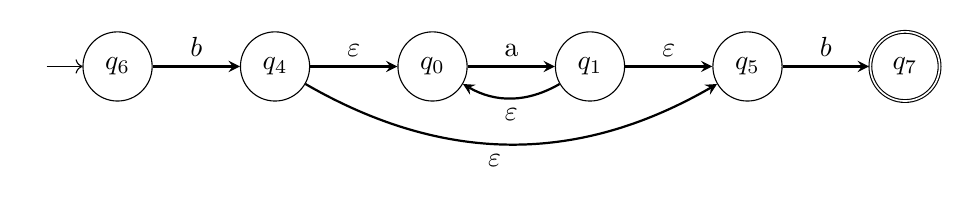
\begin{tikzpicture} [node distance = 2cm, on grid, auto]

\node (q6) [state, initial, initial text = {}] {$q_6$};
\node (q0) [state, right = of q6] {$q_4$};
\node (q1) [state, right = of q0] {$q_0$};
\node (q2) [state, right = of q1] {$q_1$};
\node (q3) [state, right = of q2] {$q_5$};
\node (q7) [state, accepting, right = of q3] {$q_7$};

\path [-stealth, thick]
        (q6) edge node {$b$}   (q0);
\path [-stealth, thick]
    (q0) edge node {$\varepsilon$}   (q1);
\path [-stealth, thick]
    (q0) edge [bend right] node[below left] {$\varepsilon$}   (q3);
\path [-stealth, thick]
    (q1) edge node {a}   (q2);
\path [-stealth, thick]
    (q2) [bend left] edge node {$\varepsilon$}   (q1);
\path [-stealth, thick]
    (q2) edge node {$\varepsilon$}   (q3);
\path [-stealth, thick]
    (q3) edge node {$b$}   (q7);

\end{tikzpicture}
\caption{Operator '$ba^*b$'} \label{fig:operatorbastarb}
\end{figure}

\begin{figure}[!htb]
\centering
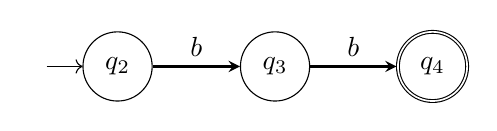
\begin{tikzpicture} [node distance = 2cm, on grid, auto]

\node (q8) [state, initial, initial text = {}] {$q_2$};
\node (q9) [state, right = of q8] {$q_3$};
\node (q4) [state, accepting, right = of q9] {$q_{4}$};

\path [-stealth, thick]
    (q8) edge node {$b$}   (q9);
\path [-stealth, thick]
    (q9) edge node {$b$}   (q4);


\end{tikzpicture}
\caption{Operator '$bb$'} \label{fig:operatorbb}
\end{figure}

\begin{figure}[!htb]
\centering
\begin{tikzpicture} [node distance = 2cm, on grid, auto]

\node (q8) [state, initial, initial text = {}] {$q_2$};
\node (q9) [state, right = of q8] {$q_3$};
\node (q0) [state, right = of q9] {$q_4$};
\node (q1) [state, right = of q0] {$q_0$};
\node (q2) [state, right = of q1] {$q_1$};
\node (q3) [state, accepting, right = of q2] {$q_5$};

\path [-stealth, thick]
    (q0) edge node {$\varepsilon$}   (q1);
\path [-stealth, thick]
    (q0) edge [bend right] node[below left] {$\varepsilon$}   (q3);
\path [-stealth, thick]
    (q1) edge node {a}   (q2);
\path [-stealth, thick]
    (q2) [bend left] edge node {$\varepsilon$}   (q1);
\path [-stealth, thick]
    (q2) edge node {$\varepsilon$}   (q3);

\path [-stealth, thick]
    (q8) edge node {$b$}   (q9);
\path [-stealth, thick]
    (q9) edge node {$b$}   (q4);
\end{tikzpicture}
\caption{Operator '$bba^*$'} \label{fig:operatorbbastar}
\end{figure}

\begin{figure}[!htb]
\centering
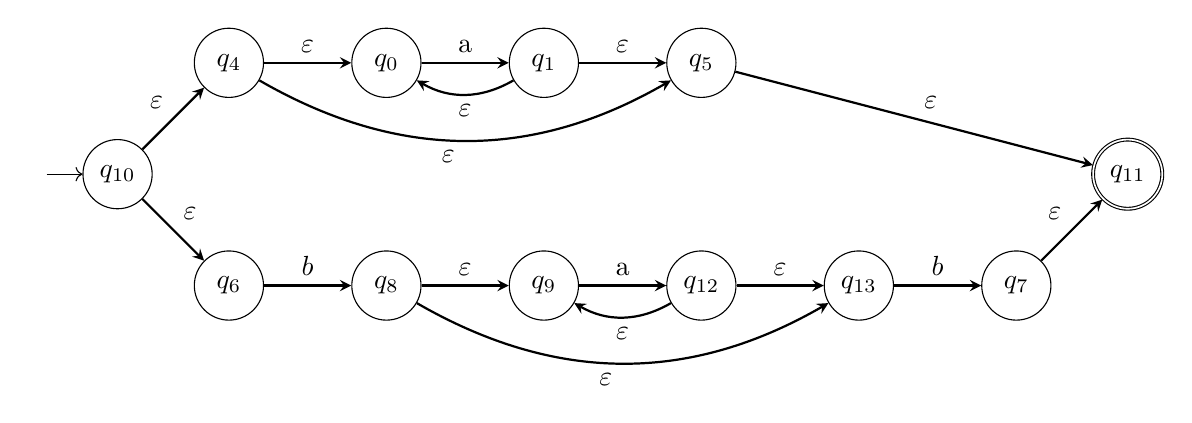
\begin{tikzpicture} [node distance = 2cm, on grid, auto]

\node (q10) [state, initial, initial text = {}] {$q_{10}$};
% a*

\node (q0) [state, above right = of q10] {$q_4$};
\node (q1) [state, right = of q0] {$q_0$};
\node (q2) [state, right = of q1] {$q_1$};
\node (q3) [state, right = of q2] {$q_5$};
% ba*b
\node (q4) [state, below right = of q10] {$q_6$};
\node (q5) [state, right = of q4] {$q_8$};
\node (q6) [state, right = of q5] {$q_9$};
\node (q7) [state, right = of q6] {$q_{12}$};
\node (q8) [state, right = of q7] {$q_{13}$};
\node (q9) [state, right = of q8] {$q_7$};

\node (q11) [state, accepting, above right = of q9] {$q_{11}$};

\path [-stealth, thick]
  (q10) edge node {$\varepsilon$}   (q0);

\path [-stealth, thick]
  (q10) edge node {$\varepsilon$}   (q4);

% a*
\path [-stealth, thick]
    (q0) edge node {$\varepsilon$}   (q1);
\path [-stealth, thick]
    (q0) edge [bend right] node[below left] {$\varepsilon$}   (q3);
\path [-stealth, thick]
    (q1) edge node {a}   (q2);
\path [-stealth, thick]
    (q2) [bend left] edge node {$\varepsilon$}   (q1);
\path [-stealth, thick]
    (q2) edge node {$\varepsilon$}   (q3);
\path [-stealth, thick]
  (q3) edge node {$\varepsilon$}   (q11);

% ba*b
\path [-stealth, thick]
        (q4) edge node {$b$}   (q5);
\path [-stealth, thick]
    (q5) edge node {$\varepsilon$}   (q6);
\path [-stealth, thick]
    (q5) edge [bend right] node[below left] {$\varepsilon$}   (q8);
\path [-stealth, thick]
    (q6) edge node {a}   (q7);
\path [-stealth, thick]
    (q7) [bend left] edge node {$\varepsilon$}   (q6);
\path [-stealth, thick]
    (q7) edge node {$\varepsilon$}   (q8);
\path [-stealth, thick]
    (q8) edge node {$b$}   (q9);
\path [-stealth, thick]
  (q9) edge node {$\varepsilon$}   (q11);
\end{tikzpicture}
\caption{Operator '$a^*+ba^*b$'} \label{fig:operatorastarOrbastarb}
\end{figure}

\begin{figure}[!htb]
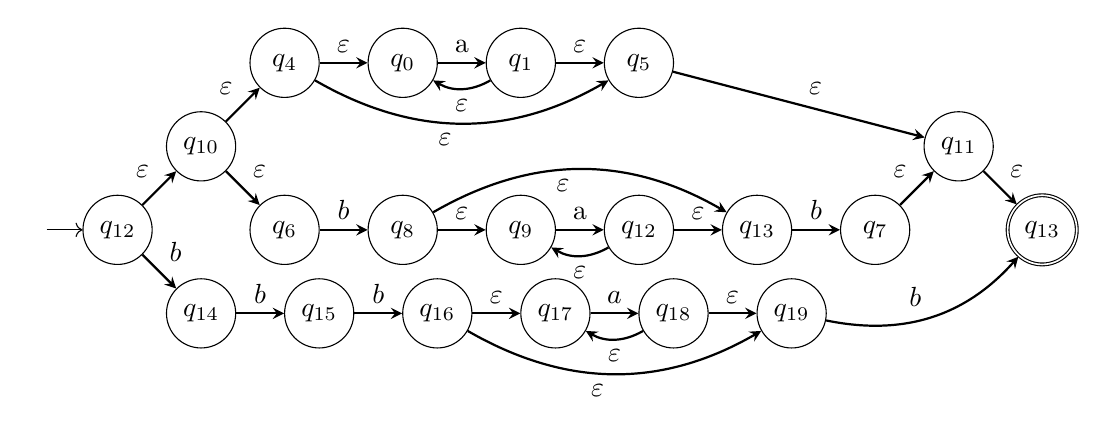
\begin{tikzpicture} [node distance = 1.5cm, on grid, auto]

\node (q12) [state, initial, initial text = {}] {$q_{12}$};

\node (q10) [state, above right = of q12] {$q_{10}$};
% a*

\node (q0) [state, above right = of q10] {$q_4$};
\node (q1) [state, right = of q0] {$q_0$};
\node (q2) [state, right = of q1] {$q_1$};
\node (q3) [state, right = of q2] {$q_5$};
% ba*b
\node (q4) [state, below right = of q10] {$q_6$};
\node (q5) [state, right = of q4] {$q_8$};
\node (q6) [state, right = of q5] {$q_9$};
\node (q7) [state, right = of q6] {$q_{12}$};
\node (q8) [state, right = of q7] {$q_{13}$};
\node (q9) [state, right = of q8] {$q_7$};

\node (q11) [state, above right = of q9] {$q_{11}$};

\node (q13) [state, accepting, below right = of q11] {$q_{13}$};

% bba*
\node (q14) [state, below right = of q12] {$q_{14}$};
\node (q15) [state, right = of q14] {$q_{15}$};
\node (q16) [state, right = of q15] {$q_{16}$};
\node (q17) [state, right = of q16] {$q_{17}$};
\node (q18) [state, right = of q17] {$q_{18}$};
\node (q19) [state, right = of q18] {$q_{19}$};

\path [-stealth, thick]
  (q12) edge node {$b$}   (q14);

\path [-stealth, thick]
  (q14) edge node {$b$}   (q15);
\path [-stealth, thick]
  (q15) edge node {$b$}   (q16);
\path [-stealth, thick]
  (q16) edge node {$\varepsilon$}   (q17);
\path [-stealth, thick]
    (q16) edge [bend right] node[below left] {$\varepsilon$}   (q19);
\path [-stealth, thick]
  (q17) edge node {$a$}   (q18);
\path [-stealth, thick]
  (q18) edge node {$\varepsilon$}   (q19);
\path [-stealth, thick]
    (q18) [bend left] edge node {$\varepsilon$}   (q17);
\path [-stealth, thick]
  (q19) edge [bend right] node {$b$}   (q13);

\path [-stealth, thick]
  (q12) edge node {$\varepsilon$}   (q10);

\path [-stealth, thick]
  (q10) edge node {$\varepsilon$}   (q0);

\path [-stealth, thick]
  (q10) edge node {$\varepsilon$}   (q4);

% a*
\path [-stealth, thick]
    (q0) edge node {$\varepsilon$}   (q1);
\path [-stealth, thick]
    (q0) edge [bend right] node[below left] {$\varepsilon$}   (q3);
\path [-stealth, thick]
    (q1) edge node {a}   (q2);
\path [-stealth, thick]
    (q2) [bend left] edge node {$\varepsilon$}   (q1);
\path [-stealth, thick]
    (q2) edge node {$\varepsilon$}   (q3);
\path [-stealth, thick]
  (q3) edge node {$\varepsilon$}   (q11);

% ba*b
\path [-stealth, thick]
        (q4) edge node {$b$}   (q5);
\path [-stealth, thick]
    (q5) edge node {$\varepsilon$}   (q6);
\path [-stealth, thick]
    (q5) edge [bend left] node[below left] {$\varepsilon$}   (q8);
\path [-stealth, thick]
    (q6) edge node {a}   (q7);
\path [-stealth, thick]
    (q7) [bend left] edge node {$\varepsilon$}   (q6);
\path [-stealth, thick]
    (q7) edge node {$\varepsilon$}   (q8);
\path [-stealth, thick]
    (q8) edge node {$b$}   (q9);
\path [-stealth, thick]
  (q9) edge node {$\varepsilon$}   (q11);
\path [-stealth, thick]
  (q11) edge node {$\varepsilon$}   (q13);

% bba*

\end{tikzpicture}
\caption{Operator '$a^*+ba^*b + bba^*$'} \label{fig:final}
\end{figure}

\begin{figure}[!htb]
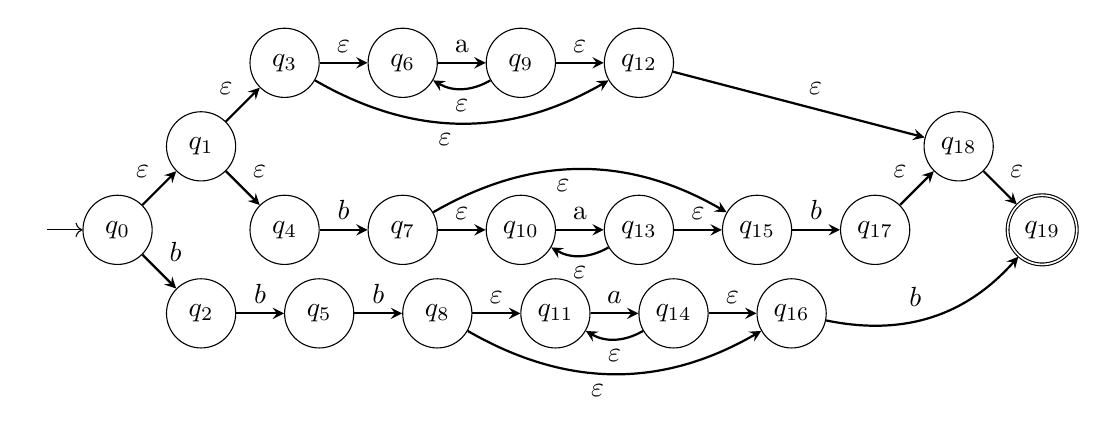
\begin{tikzpicture} [node distance = 1.5cm, on grid, auto]

\node (q12) [state, initial, initial text = {}] {$q_{0}$};

\node (q10) [state, above right = of q12] {$q_{1}$};
% a*

\node (q0) [state, above right = of q10] {$q_3$};
\node (q1) [state, right = of q0] {$q_6$};
\node (q2) [state, right = of q1] {$q_9$};
\node (q3) [state, right = of q2] {$q_{12}$};
% ba*b
\node (q4) [state, below right = of q10] {$q_4$};
\node (q5) [state, right = of q4] {$q_7$};
\node (q6) [state, right = of q5] {$q_{10}$};
\node (q7) [state, right = of q6] {$q_{13}$};
\node (q8) [state, right = of q7] {$q_{15}$};
\node (q9) [state, right = of q8] {$q_{17}$};

\node (q11) [state, above right = of q9] {$q_{18}$};

\node (q13) [state, accepting, below right = of q11] {$q_{19}$};

% bba*
\node (q14) [state, below right = of q12] {$q_{2}$};
\node (q15) [state, right = of q14] {$q_{5}$};
\node (q16) [state, right = of q15] {$q_{8}$};
\node (q17) [state, right = of q16] {$q_{11}$};
\node (q18) [state, right = of q17] {$q_{14}$};
\node (q19) [state, right = of q18] {$q_{16}$};

\path [-stealth, thick]
  (q12) edge node {$b$}   (q14);

\path [-stealth, thick]
  (q14) edge node {$b$}   (q15);
\path [-stealth, thick]
  (q15) edge node {$b$}   (q16);
\path [-stealth, thick]
  (q16) edge node {$\varepsilon$}   (q17);
\path [-stealth, thick]
    (q16) edge [bend right] node[below left] {$\varepsilon$}   (q19);
\path [-stealth, thick]
  (q17) edge node {$a$}   (q18);
\path [-stealth, thick]
  (q18) edge node {$\varepsilon$}   (q19);
\path [-stealth, thick]
    (q18) [bend left] edge node {$\varepsilon$}   (q17);
\path [-stealth, thick]
  (q19) edge [bend right] node {$b$}   (q13);

\path [-stealth, thick]
  (q12) edge node {$\varepsilon$}   (q10);

\path [-stealth, thick]
  (q10) edge node {$\varepsilon$}   (q0);

\path [-stealth, thick]
  (q10) edge node {$\varepsilon$}   (q4);

% a*
\path [-stealth, thick]
    (q0) edge node {$\varepsilon$}   (q1);
\path [-stealth, thick]
    (q0) edge [bend right] node[below left] {$\varepsilon$}   (q3);
\path [-stealth, thick]
    (q1) edge node {a}   (q2);
\path [-stealth, thick]
    (q2) [bend left] edge node {$\varepsilon$}   (q1);
\path [-stealth, thick]
    (q2) edge node {$\varepsilon$}   (q3);
\path [-stealth, thick]
  (q3) edge node {$\varepsilon$}   (q11);

% ba*b
\path [-stealth, thick]
        (q4) edge node {$b$}   (q5);
\path [-stealth, thick]
    (q5) edge node {$\varepsilon$}   (q6);
\path [-stealth, thick]
    (q5) edge [bend left] node[below left] {$\varepsilon$}   (q8);
\path [-stealth, thick]
    (q6) edge node {a}   (q7);
\path [-stealth, thick]
    (q7) [bend left] edge node {$\varepsilon$}   (q6);
\path [-stealth, thick]
    (q7) edge node {$\varepsilon$}   (q8);
\path [-stealth, thick]
    (q8) edge node {$b$}   (q9);
\path [-stealth, thick]
  (q9) edge node {$\varepsilon$}   (q11);
\path [-stealth, thick]
  (q11) edge node {$\varepsilon$}   (q13);

% bba*

\end{tikzpicture}
\caption{Operator '$a^*+ba^*b + bba^*$' - changed names of states} \label{fig:final}
\end{figure}

\section{Transforming NFA into DFA using subset algorithm}
\section{Constructing minimal state DFA}



\end{document}
